
Порождающие модели современное и быстро развивающие направление работы с данными.

Ключевыми достижениями в дисципилине были \begin{enumerate}
    \item порождающие грамматики \cite{chomsky2002syntactic}
    \item графические вероятностные модели \cite{pearl1988probabilistic}
    \item состязательные порождающие модели \cite{goodfellow2020generative}
    \item диффузионные порождающие модели \cite{song2020score}
\end{enumerate}

Порождающие модели задают совместное распределение наблюдаемого объекта $x$ и его черт $y$ -  $p(x,y)$. В этом заключается 
ключевое различие между порождающими и дискриминирующими моделями $p(y|x)$ \ref{discr_vs_gen}.

\begin{figure}[h]
    \centering
    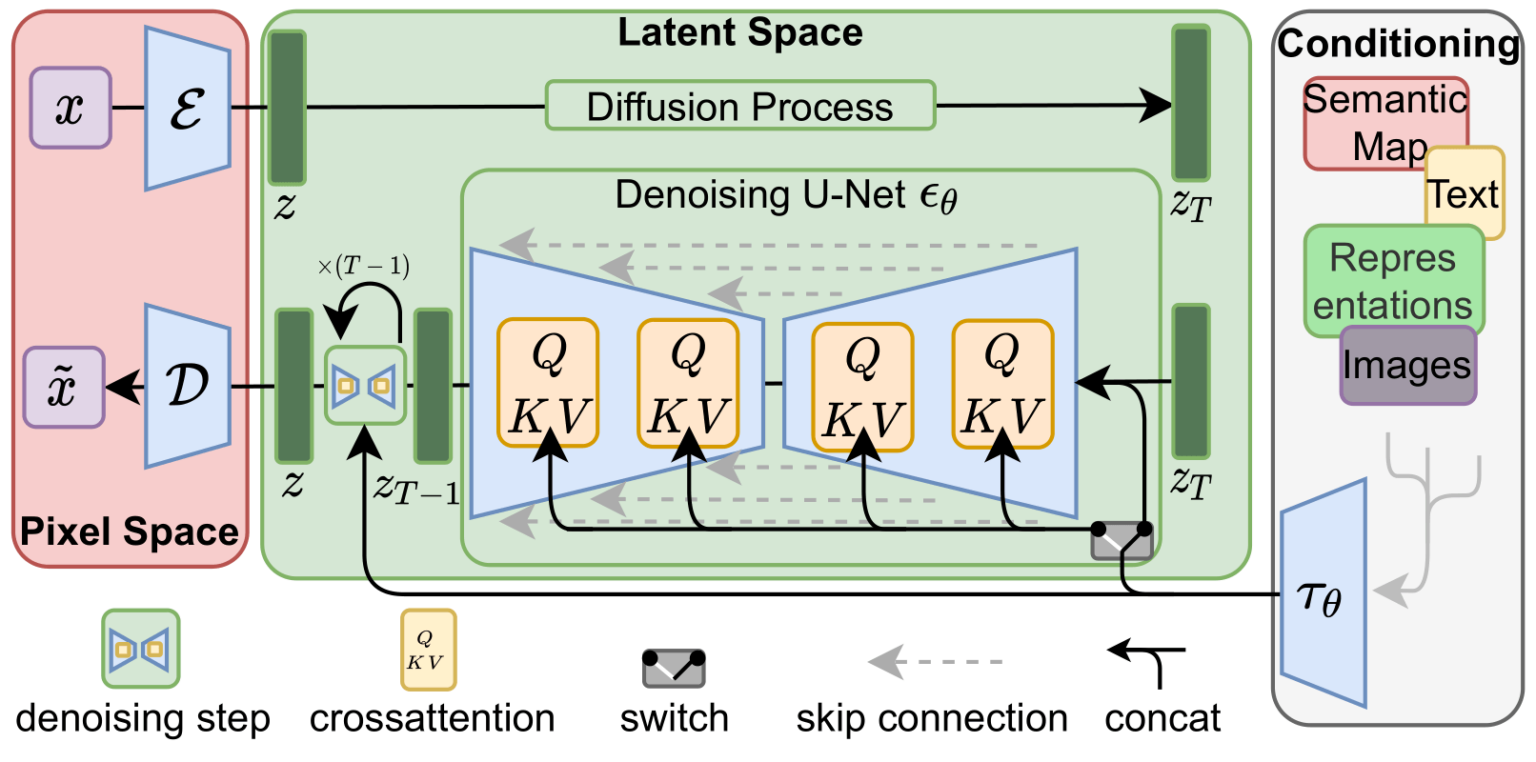
\includegraphics[width=0.5\textwidth]{assets/ml/generation/stable_diffusion.png}
    \caption{Генеративные }
    \label{discr_vs_gen}
\end{figure}

Задача 

\begin{equation}
    \mathrm E_{p(\mathbf{x})} f(\mathbf{x}) = \int p(\mathbf{x}) f(\mathbf{x}) dx \approx \frac{1}{n} \sum_i=1^n f(x_i)
\end{equation}



\textit{Определение} $f$-дивергенцией называется выпуклая функция, удовлетворяющая равенству $f(1)=0$/

$$
    D_f{\pi \parallel \rho} = \mathrm E_{\rho(x)} f\left(\frac{\pi(x)}{\rho(x)}\right)
$$

Семейство $f$-дивергенций включает функции \begin{enumerate}
    \item Кульбака-Лейбнера $f(u)=u logu $
\end{enumerate}








$$
    p(x|)
$$


особенно важным для развития генеративного моделирования.
В областях обработки естественного языка стала популярна аналитическая форма механизма внимания \cite{vaswani2017attention},
приведшая к созданию больших лингвистических моделей \cite{radford2019language}, имеющих важное практическое применение.

Неравенство Йенсена 

$$
$$





Вариационный вывод (ELBO)

$$
    \mathcal{L}(\theta)
$$


